% Run
% xelatex "\def\isarticle{1} \documentclass[10pt,a4paper]{exam}

\usepackage{tikz}
\usepackage{listings}
\lstset{language=C,inputencoding=utf8,basicstyle=\footnotesize, 
    flexiblecolumns=true, numbers=left, numberstyle=\tiny\color{gray}, 
    commentstyle=\scriptsize\color{black!50},mathescape}
  \usepackage{enumerate}
  \usepackage{lcg} % random numbers
\newcounter{exno}
\def\exercise{\addtocounter{exno}{1}\medskip\noindent{\bf Exercício \arabic{exno}.}}
\def\<#1>{\langle#1\rangle}
\def\ra{$\leftarrow$}
\def\question#1{\exercise}

\renewcommand{\lstlistingname}{Listagem}

\title{Sistemas Operacionais}
\author{}
\begin{document}

\lstset{language=C,
  basicstyle=\small,
  commentstyle={\color{gray}\tiny}
}
\date{\today}

 \lecture{Gerenciamento de Processos}{proc}

\title{Sistemas operacionais: \insertlecture}
\frame{\titlepage}

\section{\insertlecture}

% \begin{frame}
% \frametitle{O que é um processo}
% Mecanismo de controle para execução de programas que auxilia:
% \begin{itemize}
% \item Isolamento;
% \item Comunicação entre processos;
% \item Compartilhamento do processador;
% \item Interface com dispositivos de Entrada/Saída~(E/S);
% \item Gerenciamento de memória;
% \item Sincronização de recursos compartilhados.
% \end{itemize}
% \end{frame}

% \begin{frame}\frametitle{Tabela de dados}
%   \framesubtitle{Processo}
% \begin{columns}
% \begin{column}{6cm}
% \begin{small}
% A tabela de dados do processo contem o valor ou a localização:
% \begin{itemize}
% \item Identificação do processo;
% \item Código do programa em execução;
% \item Arquivos abertos;
% \item Sinais pendentes;
% % registers
% \item estado do processador;
% % address space
% % \item seção de dados contendo variáveis globais
% \item área de memória usada;
% \item Uma ou mais {\em threads} de execução.
% \end{itemize}
% \end{small}
% \end{column}

% \only<2->{
% \begin{column}{5cm}\scriptsize
% \begin{center}
%   \only<2>{Tabela de dados do processo}
%   \only<3->{Bloco de controle do processo\\({\em Process Control Block -- PCB})}
%   \smallskip
%   \def\recbase{5}
\def\recheight{1}

\begin{center}
  \begin{tikzpicture}[every rectangle/.style={minimum width=\recbase},
    scale=0.775,mem/.style={fill=gray!60},
    var/.style={fill=blue!30}]
    
    \draw[var] (0,2+5.5*\recheight) rectangle (\recbase,2+6.5*\recheight)
    node[midway] {\scriptsize{estado do processo}};
    \draw[var] (0,2+4.5*\recheight) rectangle (\recbase,2+5.5*\recheight)
    node[midway] {\scriptsize{número do processo}};
    \draw[var] (0,2+3.5*\recheight) rectangle (\recbase,2+4.5*\recheight)
    node[midway] {\scriptsize{contador de programa}};
    \draw[mem] (0,2+2*\recheight) rectangle (\recbase,2+3.5*\recheight) node[midway] {registradores};
    \draw[var] (0,2+\recheight) rectangle (\recbase,2+2*\recheight) node[midway] {limites de
    memória};
    \draw[var] (0,1.5) rectangle (\recbase,2+\recheight) node[midway] {\scriptsize{lista de
    arquivos abertos}};
    \draw[mem] (0,0) rectangle (\recbase,1.5*\recheight) node[midway] {$\ldots$};
  \end{tikzpicture}
\end{center}

% \end{center}
% \end{column}
% } 
% \end{columns}
% \end{frame}

% \subsection{Estados dos processos}

% \begin{frame}{Estados de um processo}
  
% \begin{block}{Estados}
%   \begin{description}
%   \item[Novo] O processo está sendo criado.
%   \item[Executando] As instruções estão sendo executadas.
%   \item[Esperando] O processo está esperando pela ocorrência de algum
%     evento (como um término de E/S ou um sinal).
%   \item[Pronto] O processo está esperando para ser designado a um processador.
%   \item[Terminado] O processo terminou sua execução.
%   \end{description}
% \end{block}

% \end{frame}

% \begin{frame}[fragile]{Transição dos estados de um processo}
  
% 	\makeatletter
\colorlet{new}{white}
\colorlet{ready}{blue}
\colorlet{exec}{red}
\colorlet{wait}{orange!70!black}
\colorlet{end}{black}

  \begin{center}
    \begin{tikzpicture}[every node/.style={font=\scriptsize},
      state/.style={ellipse,font=\bf,draw},
      transition/.style={->,>=latex},
      statelabel/.style={midway,font=\bf\tiny,text width=1.5cm,align=center}]
      \def\@@ds{1.75cm}
      \node[fill=new,draw] (new) at (0,0) {\bf\large novo};
      \node[above of=new,yshift=-.5cm] {\footnotesize\tt cria PCB};
      \node[color=white,state,fill=ready] (ready) at (2*\@@ds,-\@@ds) {pronto};
      \node[color=yellow,state,fill=exec] (exec) at (4*\@@ds,0) {executando};
      \node[color=gray!30,state,fill=wait] (wait) at (2*\@@ds,\@@ds) {esperando};
      \node[white,fill=black] (end) at (4.5*\@@ds,\@@ds) {t\'ermino};
      \node[above of=end,yshift=-.35cm] {\footnotesize\tt apaga PCB};
    
      \draw[transition,draw=ready] (new) .. controls +(down:8mm) and +(left:32mm) .. (ready)  node[statelabel,left] {enviado para a fila};
      \draw[transition,draw=exec] (ready) .. controls +(right:32mm) and +(down:8mm) .. (exec)  node[statelabel,right] {escalonado para execu\c{c}\~ao};
      \draw[transition,draw=ready] (exec.west) .. controls +(left:8mm) and +(up:8mm) .. (ready.north)  node[statelabel,above] {escalonado para a fila};
      \draw[transition,draw=wait] (exec.north) .. controls +(up:16mm) and +(right:4mm) .. (wait.east) node[statelabel,above] {requisi\c{c}\~ao E/S};
      \draw[transition,draw=ready] (wait.west) .. controls +(left:16mm) and +(left:16mm) .. (ready.west) node[statelabel,right] {t\'ermino E/S};
      \draw[transition,draw=end] (exec) .. controls +(right:32mm) and +(right:24mm) .. (end) node[statelabel,left] {t\'ermino do processo};
      
    \end{tikzpicture}

  \end{center}
  \makeatother

% \end{frame}

% \begin{frame}{Sequência dos PCBs}{Transição de estados}

% \begin{center}
% 	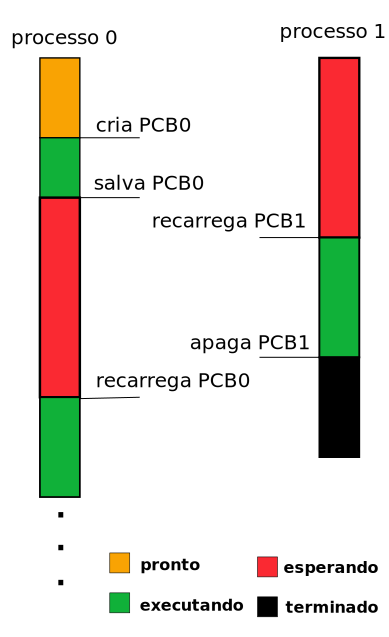
\includegraphics[scale=0.45]{pcb-sequence}
% \end{center}
% \end{frame}

% \subsection{Criação de um processo}

% % A criação de processos em sistemas derivados do Unix usa a função
% % \lstinline{fork()}, que geralmente segue as seguintes etapas:

% % \begin{enumerate}
% % \item Cria a tabela de dados do processo;
% % \item Checa os limites do processo;
% % \item Inicializa a tabela de dados;
% % \item Atribui um número de identificação do processo;
% % % Duplica (Processo -> COW), compartilha (Threads)
% % \item ``Duplica'' ou compartilha:
% %   \begin{itemize}
% %   \item Arquivos abertos;
% %   \item Sistema de arquivos;
% %   \item Espaço de endereçamento (memória);
% %   \item Sinais.
% %   \end{itemize}
% % \end{enumerate}
% \lstset{emph={%  
%     fork, wait, exit%
%     },emphstyle={\color{red}\bfseries\underbar}%
% }%
% \begin{frame}[fragile]
%   \frametitle{Criação de um processo}
%   \framesubtitle{Derivados do Unix: \lstinline{fork()}}
%   \begin{columns}
%     \begin{column}{.6\textwidth}\scriptsize
% \noindent Fragmento de código para %
% criação de processo.\\\bigskip      
% \begin{lstlisting}
% int pid = fork();
% if(pid > 0){
%     printf("proc-pai: filho=%d\n", pid);
%     pid = wait((int *) 0);
%     printf("proc-filho %d terminou\n", pid);
% } else if(pid == 0){
%     printf("proc-filho: saindo\n");
%     exit(0);
% } else {
%     printf("erro\n");
% }
% \end{lstlisting}
% \end{column}
%     \begin{column}{.4\textwidth}
%       \includegraphics[scale=.525]{fork.png}
%     \end{column}
%   \end{columns}

%   %\hfill
%   %\noindent $^\star$ {\tiny Fonte: {\tt https://pdos.csail.mit.edu/6.S081/2020/xv6/book-riscv-rev1.pdf}}
% \end{frame}

% %%%%%%%%%%%%%%%%%%%%%%%%%%%%%%%%%%%%%%%%%%%%%%%%%%%%%%%%%%%%%%%%
% %% BUFFER
% %%%%%%%%%%%%%%%%%%%%%%%%%%%%%%%%%%%%%%%%%%%%%%%%%%%%%%%%%%%%%%%%

% \ifnum1=2
% \begin{frame}{Exemplos e aplicações}

%   \begin{itemize}
%     \item \href{http://lxr.linux.no/\#linux+v2.6.37.1/include/linux/sched.h\#L1182}{Analisar os membros da estrutura de {\tt task\_struct}}
%   \item Monitoramento de processos usando as ferramentas do Linux {\tt
%       ps}, {\tt top}, {\tt atop}, {\tt htop}.
%   \item \href{http://adrianoholanda.org/edu/file.php/3/codigo_fonte/proc_cria_posix.c}{Criação
%       de processos utilizando a API Posix.}
%   \item \href{http://adrianoholanda.org/edu/file.php/3/codigo_fonte/proc_cria_win32.c}{Criação
%       de processos usando chamadas de sistema do Windows.}
%   \end{itemize}
  
% \end{frame}
% \fi

%%% Local Variables: 
%%% mode: latex
%%% TeX-master: main
%%% End: 

 %%% Local Variables:
%%% mode: xelatex
%%% TeX-master: "main"
%%% End:

\section*{Concorrência e Sincronização}

\exercise~As threads 0 ($T_0$) e 1 ($T_1$) acessam a variável global
$i$ com concorrência, incrementando seu valor com a expressão {\tt
  i++} da linguagem C. Supondo que o valor inicial de $i$ seja $8$, o
valor final de $i$ após a execução das 2 threads deve ser $10$. Se a
conversão da expressão para uma liguagem de montagem hipotética gerar
o seguinte código:

\begin{verbatim}
        LOAD      R1,#i      # 0. Lê o contéudo de i e escreve no registrador R1.
        ADD       R1,R1,1    # 1. Incrementa o valor contido em R1.
        STORE     R1,#i      # 2. Escreve o conteúdo de R1 em i.
\end{verbatim}

\noindent e tomarmos a convenção de que a tupla $\<T_0,1>$ indica
a execução da linha 1 da thread 0, calcule o valor final de $i$ após a
execução das seguintes sequências de instruções:

\begin{enumerate}[a)]
\item $\<T_0,0> \rightarrow \<T_0,1> \rightarrow \<T_0,2>
\rightarrow\<T_1,0>\rightarrow\<T_1,1> \rightarrow\<T_1,2>$
\item $\<T_0,0> \rightarrow\<T_1,0> \rightarrow\<T_0,1>
\rightarrow\<T_1,1>\rightarrow\<T_0,2> \rightarrow\<T_1,2>$
\item $\<T_0,0>\rightarrow\<T_0,1> \rightarrow\<T_1,0>
\rightarrow\<T_1,1>\rightarrow\<T_0,2> \rightarrow\<T_1,2>$
\item $\<T_1,0>\rightarrow\<T_1,1> \rightarrow\<T_0,0>
\rightarrow\<T_0,1>\rightarrow\<T_0,2> \rightarrow\<T_1,2>$
\item $\<T_1,0>\rightarrow\<T_1,1>\rightarrow\<T_1,2>
\rightarrow\<T_0,0>\rightarrow\<T_0,1>\rightarrow\<T_0,2>$
\end{enumerate}

\noindent Quais das sequências enumeradas garante que o valor final de $i$ seja
íntegro? O que pode ser feito para garantir que o valor final de $i$
seja igual ao valor esperado?

\exercise~As primitivas de exclusão mútua podem ser implementadas com
espera ociosa ou com bloqueio. Discuta a aplicabilidade e os méritos
relativos de cada abordagem.

\exercise~Explique como a habilitação e a desabilitação de
interrupções são úteis na implementação de primitivas de exclusão
mútua em sistemas com um único processador.

\exercise~Verifique se a implementação de {\em spin lock} usando a
função {\tt sincroniza0()} a seguir é confiável para a sincronização
das {\em threads} 0 e 1. Explique detalhadamente a verificação.\bigskip

\begin{minipage}{.48\textwidth}
\begin{lstlisting}
  /* Thread 0 */
  int haBloqueio;
  void sincroniza0() {
    while (haBloqueio == 1) {/* spin */};
    haBloqueio = 1;
    /* região crítica */
    haBloqueio = 0;
  }
\end{lstlisting}
\end{minipage}
\begin{minipage}{.48\textwidth}
\begin{lstlisting}
  /* Thread 1 */
  int haBloqueio;
  void sincroniza0() {
    while (haBloqueio == 1) {/* spin */};
    haBloqueio = 1;
    /* região crítica */
    haBloqueio = 0;
  }
\end{lstlisting}
\end{minipage}

\exercise~Verifique se a implementação de {\em spin lock} usando a
função {\tt sincroniza1(int tid)} a seguir é confiável para a
sincronização das {\em threads} 0 e 1. Explique detalhadamente a
verificação.\bigskip

\begin{minipage}{.48\textwidth}
\begin{lstlisting}
  /* Thread 0 */
  int vez;
  void sincroniza1(int tid) {/* passado valor 0 */
    /* tid é a identificação da thread */
    while (vez == 1-tid) {/* spin */};
    vez = tid;
    /* região crítica */
    vez = 1  - tid;
  }
\end{lstlisting}
\end{minipage}
\begin{minipage}{.48\textwidth}
\begin{lstlisting}
  /* Thread 1 */
  int vez;
  void sincroniza1(int tid) {/* passado valor 1 */
    /* tid é a identificação da thread */
    while (pid == 1 - tid) {/* spin */};
    vez = tid;
    /* região crítica */
    vez = 1 - tid;
  }
\end{lstlisting}
\end{minipage}

\exercise~Mostre que o algoritmo de Peterson limita o tempo de cada
thread com justiça, ou seja, uma thread não pode ser atrasada
indefinidamente em qualquer condição de espera. Em particular, mostre
que qualquer thread que esteja a espera para entrar em sua região
crítica será atrasada por não mais do que o tempo que a outra thread
leva para entrar e sair de sua região crítica uma vez.

% \exercise~Apresente uma análise detalhada do Algoritmo de Peterson
% para demonstrar que funciona adequadamente. Em particular, mostre se
% há ocorrência de impasse (deadlock) ou espera indefinida, e que a
% exclusão mútua é imposta com sucesso.

\exercise~Leia os artigos da Wikipédia buscando a palavra ``Dijkstra''
e pelo verbete ``Semáforo (computação)''. Verifique quais são as
referências de cada artigo e ligações externas (se houver).


\ifnum1=2

\section{Sincronização}
\subsection{Exercícios}

Em uma aplicação concorrente que controla saldo bancário em contas
correntes, dois processoscompartilham uma região de memória onde estão
armazenados os saldos dos clientes A e B. Osprocessos executam,
concorrentemente os seguintes passos: 

\begin{figure}[h]
\begin{tt}
\begin{tabular}{l|l}
Processo 1 (Cliente A) & Processo 2 (Cliente B) \\
\/\* saque em A */ & /* saque em A */ \\
1a. x \ra{} saldo\_do\_cliente\_A; & 2a. y \ra{} saldo\_do\_cliente\_A; \\
1b. x \ra{} x - 200; & 2b. y \ra{} y - 100;\\
1c. saldo\_do\_cliente\_A \ra{} x; & 2c. saldo\_do\_cliente\_A \ra{} y;\\
/* deposito em B */ & /* deposito em B */\\
1d. x \ra{} saldo\_do\_cliente\_B; & 2d. y \ra{} saldo\_do\_cliente\_B;\\
1e. x \ra{} x + 100; & 2e. y \ra{} y + 200;\\
1f. saldo\_do\_cliente\_B \ra{} x; & 2f. saldo\_do\_cliente\_B \ra{} y; \\
\end{tabular}
\end{tt}
\caption{Acesso concorrente à atualização de conta bancária.}
\end{figure}

Supondo que os valores dos saldos de A e B sejam, respectivamente, 500
e 900, antes de os processosexecutarem, pede-se:

\begin{itemize}
\item Quais os valores corretos esperados para os saldos dos clientes
  A e B após o término da execuçãodos processos?\\

R: Cliente A = 200 e Cliente B = 1.200

\item Quais os valores finais dos saldos dos clientes se a sequência
  temporal de execução das operaçõesfor: 1a, 2a, 1b, 2b, 1c, 2c, 1d,
  2d, 1e, 2e, 1f, 2f?\\

R: Cliente A = 400 e Cliente B = 1.100

\item Utilizando semáforos, proponha uma solução que garanta a
  integridade dos saldos e permita o maiorcompartilhamento possível
  dos recursos entre os processos, não esquecendo a especificação
  dainicialização dos semáforos.
\end{itemize}

\begin{figure}
\centering
\begin{tt}
\begin{tabular}{l|l}
Processo 1 (Cliente A) & Processo 2 (Cliente B)\\
/* saque em A */ & /* saque em A */\\
Down (S1) & Down (S1)\\
x \ra{} saldo\_do\_cliente\_A; & y \ra{} saldo\_do\_cliente\_A;\\
x \ra{} x - 200; & y \ra{} y - 100; \\ 
saldo\_do\_cliente\_A \ra{} x; &  saldo\_do\_cliente\_A \ra{} y;\\
Up (S1) & Up (S1)\\
/* deposito em B */ & /* deposito em B */\\
Down (S2) & Down (S2)\\
x \ra{} saldo\_do\_cliente\_B; & y \ra{} saldo\_do\_cliente\_B;\\
x \ra{} x + 100; & y \ra{} y + 200;\\
saldo\_do\_cliente\_B \ra{} x; & saldo\_do\_cliente\_B \ra{} y;\\
Up (S2) & Up (S2) \\ 
\end{tabular}
\end{tt}

\caption{Acesso concorrente utilizando semáforo para evitar inconsistências.}
\end{figure}


O problema dos leitores/escritores, apresentado a seguir, consiste em
sincronizar processos queconsultam/atualizam dados em uma base
comum. Pode haver mais de um leitor lendo ao mesmo tempo;no entanto,
enquanto um escritor está atualizando a base, nenhum outro processo
pode ter acesso a ela(nem mesmo leitores).

\begin{tt} 
\begin{tabbing}
  VAR \=Acesso: Semaforo := 1;\\
  \>Exclusao: Semaforo := 1;\\
  \>Nleitores: integer := 0;\\

PROCEDURE Escritor;\\
BEGIN\\
\> ProduzDado;\\
\> DOWN (Acesso);\\
\> Escreve;\\
\> UP (Acesso);\\
END;\\

PROCEDURE Leitor;\\
BEGIN\\
\> DOWN (Exclusao);\\
\> Nleitores := Nleitores + 1;\\
\> IF ( Nleitores = 1 ) THEN DOWN (Acesso);\\
\> UP (Exclusao);\\
\> Leitura;\\
\> DOWN (Exclusao);\\
\> Nleitores := Nleitores - 1;\\
\> IF ( Nleitores = 0 ) THEN UP (Acesso);\\
\> UP (Exclusao);\\
\> ProcessaDado;
END;\\
 
\end{tabbing}
\end{tt}
 
\begin{itemize}
 
\item Suponha que exista apenas um leitor fazendo acesso à
  base. Enquanto este processo realiza aleitura, quais os valores das
  três variáveis?  

  R: Acesso=0 Exclusao=1 Nleitores=1
 
\item Chega um escritor enquanto o leitor ainda está lendo. Quais os
  valores das três variáveis após obloqueio do escritor ? Sobre
  qual(is) semáforo(s) se dá o bloqueio?  

R: Acesso=0 Exclusao=1 Nleitores=1, o bloqueio ocorre no semáforo
Acesso.
 
\item Chega mais um leitor enquanto o primeiro ainda não acabou de ler
  e o escritor está bloqueado.Descreva os valores das três variáveis
  quando o segundo leitor inicia a leitura.  

R: Acesso=0 Exclusao=1 Nleitores=2
 
\item Os dois leitores terminam simultaneamente a leitura. É possível
  haver problemas quanto àintegridade do valor da variável nleitores?
  Justifique.  

R: Não, pois a exclusão mútua a esta variável é implementada pelo
semáforo Exclusao.
 
\item Descreva o que acontece com o escritor quando os dois leitores
  terminam suas leituras. Descrevaos valores das três variáveis quando
  o escritor inicia a escrita.  
  
  R: O processo Escritor inicia a escrita. Acesso=0 Exclusao=1
  Nleitores=0
 
\item Enquanto o escritor está atualizando a base, chagam mais um
  escritor e mais um leitor. Sobrequal(is) semáforo(s) eles ficam
  bloqueados? Descreva os valores das três variáveis após obloqueio
  dos recém-chegados.  

R: Os processo ficam bloqueados no semáforo Acesso. Acesso=0
Exclusao=0 Nleitores=1
 
\item Quando o escritor houver terminado a atualização, é possível
  prever qual dos processosbloqueados (leitor ou escritor) terá acesso
  primeiro à base?  

R: Não, em geral os sistemas operacionais utilizam a escolha randômica
dentre os processos em estado deespera.
 
\item Descreva uma situação onde os escritores sofram starvation
  (adiamento indefinido).  

  R: Caso um processo Escritor esteja aguardando, bloqueado pelo
  semáforo Acesso, e sempre surgirem novosprocessos Leitor, o processo
  Escritor pode nunca ganhar acesso ao recurso.
\end{itemize}

\end{document}
\fi


  \question[3] Dois processos acessam a variável global {\tt
    numero\_de\_acessos}, que indica o número de acessos em uma página
  web, de acordo com as instruções a seguir:
  
  \begin{tt}
  \begin{center}
    \begin{tabular}{|l|}\hline
      \bf Processo 0\\\hline
      0a. x $\leftarrow$ numero\_de\_acessos\\
      0b. x $\leftarrow$ x + 10\\
      0c. numero\_de\_acessos $\leftarrow$ x\\\hline
    \end{tabular}
  \end{center}
\end{tt}

\begin{tt}
  \begin{center}
    \begin{tabular}{|l|}\hline
      \bf Processo 1\\\hline
      1a. y $\leftarrow$ numero\_de\_acessos\\
      1b. y $\leftarrow$ y + 18\\
      1c. numero\_de\_acessos $\leftarrow$ y\\\hline
    \end{tabular}
  \end{center}
\end{tt}

\reinitrand[counter=rand,first=128,last=2048] 

Supondo que o valor inicial da variável {\tt numero\_de\_acessos} é
\rand{\arabic{rand}}, responda as seguintes questões:

\begin{parts}

\part 
Qual o valor esperado para a variável {\tt numero\_de\_acessos},
se a execução for sequencial, com o {\tt Processo 0} executando
primeiro?

\part
\label{unsync} Se o acesso não for sequencial, mas concorrente,
qual o valor final da variável {\tt numero\_de\_acessos} se a
sequência temporal de execução for {\tt 0a, 1a, 0b, 1b, 0c, 1c}?

\part Se houver inconsistência no valor esperado para {\tt
  numero\_de\_acessos} após a execução da sequência descrita no item
\ref{unsync}, como ela poderia ser consertada utilizando os
mecanismos de sincronização? Demonstre como seria o código
corrigido.

\end{parts}

  \question[1] Qual a diferença básica entre os mecanismos de
  sincronização {\bf \em spin lock} e {\em \bf mutex}? Para as
  características ou requisitos dos processos listados na tabela,
  escolha qual mecanismo é mais adequado para sincronização.
  \bigskip
  \def\whichlock{( ) {\em spin lock}\hbox{     } ( ) {\em mutex}}
  \begin{table}[h]
    \centering
    \begin{tabular}{|c|c|}\hline
      \bf Característica/Requisito & \bf Bloqueio recomendado\\\hline\hline
      Baixa sobrecarga de bloqueio & \whichlock\\\hline
      Tempo curto de bloqueio & \whichlock\\\hline
      Tempo longo de bloqueio & \whichlock\\\hline
      Necessidade de espera durante a posse do bloqueio & \whichlock\\\hline
    \end{tabular}
    \caption{Bloqueio recomendado de acordo com as características do
      bloqueio do processo.}
    \label{so:sync}
  \end{table}


\question[3] O algoritmo de Peterson pode ser usado para implementar
o mecanismo de bloqueio do tipo {\em spin} ({\em spin lock}), que evita
que duas {\em threads} ou processos interessados no mesmo recurso entrem
na região crítica ao mesmo tempo. O algoritmo em {\sc C} é listado a seguir:

\lstset{numbers=left,numberstyle=\scriptsize,
        commentstyle=\footnotesize\color{gray},
        frame=single}
\begin{lstlisting}
int vez; 
int interessado[2]; 

void Peterson(int tid) { 
     int outro; 
     outro = 1 - tid; 

     interessado[tid] = 1; 
     vez = tid; 

     while(vez == tid && interessado[outro] == 1)
                /* laço infinito */;

     /* REGIÃO CRÍTICA */

     interessado[tid] = 0;
}
\end{lstlisting}

\noindent O argumento {\tt int tid} recebe o valor 0 ou 1, indicando em qual das
2 {\em threads} o algoritmo está sendo executado.

Vamos adotar a seguinte convenção: $T_{n,m}$ indica que a {\em thread}
$n$ está executando a linha $m$ do código. Por exemplo, $T_{0,9}$
indica que a {\em thread} $0$ executa a linha $9$, ou seja, {\tt vez =
0}.

Realize as sequências a seguir, e indique qual {\em thread} entrará na
região crítica e qual {\em thread} ficará esperando no laço infinito.

\begin{enumerate}[a)]

\item $T_{0,5}$, $T_{0,6}$, $T_{0,8}$, $T_{0,9}$, $T_{1,5}$, $T_{1,6}$,
$T_{1,9}$, $T_{0,11}$, $T_{1,11}$;

\item $T_{1,5}$, $T_{1,6}$, $T_{1,8}$, $T_{1,9}$, $T_{0,5}$, $T_{0,6}$,
$T_{0,9}$, $T_{0,11}$, $T_{1,11}$;

\end{enumerate}

O que acontece se as duas {\em threads} executarem a linhas $11$ ao
mesmo tempo?

 
\lecture{Deadlock (impasse)}{deadlock}

\frame{\title{\insertlecture}\maketitle}

\section{\insertlecture}
\begin{frame}{\insertlecture}
  \def\A{{\color{brown}A}}
  \def\B{{\color{blue}B}}
  \def\dist{15mm}
  \def\waiting{{\color{red} esperando...}}
    \begin{tikzpicture}[memory/.style={rectangle,draw,very thick,anchor=east,font=\footnotesize},
    op/.style={rectangle,very thick,font=\scriptsize}]
    \node (mem1) [memory] {\A};
    \node (mem2) [memory, right of=mem1] {\B};

    \node (t1) [right of=mem1,xshift=\dist] {{\em Thread} $1$};
    \node (t1op1) [below of=t1,op,yshift=1mm] {{\tt bloqueia(\A)}};
    \node (t1op2) [below of=t1op1,op] {sucesso: realiza bloqueio em
{\tt A}!!};
    \node (t1op3) [below of=t1op2,op] {{\tt bloqueia(\B)}};
    \node (t1op4) [below of=t1op3,op] { falha, \waiting};
    \node (t1op5) [below of=t1op4,op] {\waiting};
    \node (t1op6) [below of=t1op5,op] {\waiting};

    \node (t2) [right of=t1, xshift=3*\dist] {{\em Thread} $2$};
    \node (t2op1) [below of=t2,op] {{\tt bloqueia(\B)}};
    \node (t2op2) [below of=t2op1,op] {sucesso: realiza bloqueio em
{\tt B}!!};
    \node (t2op3) [below of=t2op2,op] {{\tt bloqueia(\A)}};;
    \node (t2op4) [below of=t2op3,op] {falha, {\color{red} esperando...}};
    \node (t2op5) [below of=t2op4,op] {\waiting};
    \node (t2op6) [below of=t2op5,op] {\waiting};

    \path (t1) edge[->] (t1op1);
    \path (t1op1) edge[->] (t1op2);
    \path (t1op2) edge[->] (t1op3);
    \path (t1op3) edge[->] (t1op4);
    \path (t1op4) edge[->] (t1op5);
    \path (t1op5) edge[->] (t1op6);

    \path (t2) edge[->] (t2op1);
    \path (t2op1) edge[->] (t2op2);
    \path (t2op2) edge[->] (t2op3);
    \path (t2op3) edge[->] (t2op4);
    \path (t2op4) edge[->] (t2op5);
    \path (t2op5) edge[->] (t2op6);
  \end{tikzpicture}

\end{frame}

\begin{frame}[fragile]{Exemplo de código com possível deadlock}
\lstset{emph={MUTEX1},emphstyle={\color{blue}},
emph={[2]mutex0},emphstyle={[2]\color{red}},
language=C,basicstyle=\scriptsize}  

\begin{lstlisting}
  mutex_t mutex0, MUTEX1;
\end{lstlisting}

\lstset{frame=single}
\begin{columns}
    \begin{column}{.5\textwidth}
      \begin{block}{Thread 0}
      \begin{lstlisting}
        mutex_lock(&mutex0);
        mutex_lock(&MUTEX1);
        /**
        * região crítica
        */
        mutex_unlock(&MUTEX1);
        mutex_unlock(&mutex0);
      \end{lstlisting}
    \end{block}
  \end{column}
  \begin{column}{.5\textwidth}
    \begin{block}{Thread 1}
      \begin{lstlisting}
        mutex_lock(&MUTEX1);
        mutex_lock(&mutex0);
        /**
        * região crítica
        */
        mutex_unlock(&mutex0);
        mutex_unlock(&MUTEX1);
      \end{lstlisting}
    \end{block}
  \end{column}
\end{columns}


\end{frame}

\begin{frame}{Grafo de alocação de recursos}
  
  \begin{columns}

    \begin{column}{0.5\textwidth}


      {\footnotesize P -- processo \\ R -- recurso \\ A -- arcos \\
        $P\rightarrow R$, processo $P$ requisita recurso $R$\\
        $R\rightarrow P$, recurso $R$ é atribuído para $P$\bigskip}

      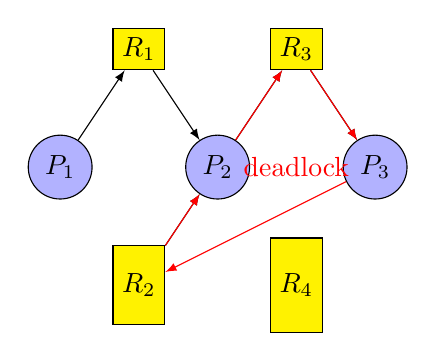
\begin{tikzpicture}
        \tikzset{proc/.style={circle,draw,fill=white!70!blue},
          res/.style={rectangle,draw,fill=yellow}}

        \foreach \x in {1,2,3}
        \node[proc] (p\x) at (2*\x,0) {$P_\x$};
        \foreach \x in {1,3}
        \node[res] (r\x) at (2+\x,1.5) {$R_\x$};
        \node[res,minimum height=1cm] (r2) at (3,-1.5) {$R_2$};
        \node[res,minimum height=1.2cm] (r4) at (5,-1.5) {$R_4$};

        \draw[->,>=latex] (p1) -- (r1);
        \draw<1>[->,>=latex] (p2) -- (r3);
        \draw<2>[->,>=latex,color=red] (p2) -- (r3);
        \draw[->,>=latex] (r1) -- (p2);
        \draw<1>[->,>=latex] (r2) -- (p2);
        \draw<2>[->,>=latex,color=red] (r2) -- (p2);
        \draw<1>[->,>=latex] (r3) -- (p3);
        \draw<2>[->,>=latex,color=red] (r3) -- (p3);
        \draw<2>[->,>=latex,color=red] (p3) -- (r2);

        \node<2>[color=red] at (5,0) {deadlock};

      \end{tikzpicture}

      \end{column}
      \begin{column}{0.35\textwidth}
              Representação\\

        \small
        \begin{tabbing}
        $P =$ \= $\{P_1, P_2, P_3\}$\\
        $R =$ \> $\{R_1, R_2, R_3, R_4\}$\\
        $\vec{A} =$ \> $\{$\=$\{P_1,R_1\}, \{P_2, R_3\},$ \\
        \>\> $\{R_1,P_2\}, \{R_2,P_2\},$ \\
        \>\> $\{R_2,P_1\}, \{R_3,P_3\}$\only<2>{$,$}\only<1>{$\}$}\\
        \>\> \only<2>{{\color{red}$\{P_3,R_2\}\}$}}\\
      \end{tabbing}
      Se um grafo não tiver ciclo não possui {\em deadlock}.
    \end{column}

  \end{columns}

\end{frame}



%\ifnum1=2%%%%%%%%%%%%%%%%%%%%%%%%%%%%%%%%BUFFER

\begin{frame}{Grafo de alocação com ciclo}{Vários recursos}
  \small
  Um ciclo pode ser eliminado com a liberação de um recurso e o {\em deadlock} é desfeito.

  \begin{center}
        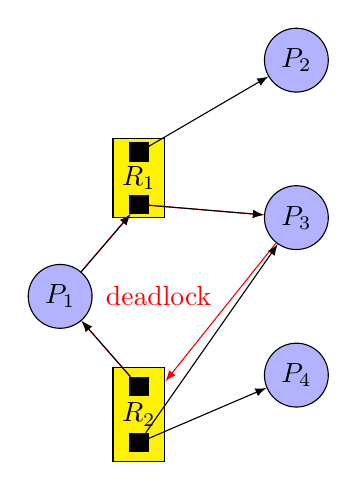
\begin{tikzpicture}
        \tikzset{proc/.style={circle,draw,fill=white!70!blue},
          res/.style={rectangle,draw,fill=yellow}}


        \node[proc] (p1) at (0,0) {$P_1$};
        \node[proc] (p2) at (3,3) {$P_2$};
        \node[proc] (p3) at (3,1) {$P_3$};
        \node[proc] (p4) at (3,-1) {$P_4$};
        \node[res,minimum height=1cm] (r1) at (1,1.5) {$R_1$};
        \node[res,minimum height=1.2cm] (r2) at (1,-1.5) {$R_2$};
        \node[fill,draw] (R11) at (r1.north)[yshift=-.175cm] {};
        \node[fill,draw] (R12) at (r1.south)[yshift=.175cm] {};
        \node[fill,draw] (R21) at (r2.north)[yshift=-.25cm] {};
        \node[fill,draw] (R22) at (r2.south)[yshift=.25cm] {};

        \draw<1>[->,>=latex,color=red] (p1) -- (R12);
        \draw<2>[->,>=latex] (p1) -- (R12);
        \draw[->,>=latex] (R11) -- (p2);
        \draw<1>[->,>=latex,color=red] (R21) -- (p1);
        \draw<2>[->,>=latex] (R21) -- (p1);
        \draw<1>[->,>=latex,color=red] (R12) -- (p3);
        \draw<2>[->,>=latex] (R12) -- (p3);
        \draw<1>[->,>=latex,color=red] (p3) -- (r2);
        \draw<2>[->,>=latex] (R22) -- (p3);

        \draw<1>[->,>=latex] (R22) -- (p4);

        \node<1>[color=red] at (1.25,0) {deadlock};

      \end{tikzpicture}
    \end{center}
    \only<2>{Quando $P_4$ libera o recurso acaba o {\em deadlock}}

\end{frame}

\begin{frame}{Solução para recursos com N objetos cada}

  \begin{itemize}
  \item Algoritmo do banqueiro (Dijkstra)
  \end{itemize}
  
\end{frame}

\begin{frame}{$+$Sincronização}
  \begin{itemize}
  \item Jantar dos filósofos;
  \item Monitores;
  \item Algoritmo do banqueiro.
  \end{itemize}

\end{frame}

%\fi

 %% Local variables:
%% mode: latex
%% TeX-master: main
%% TeX-engine: xelatex
%% End:
\footnotesize

\exercise~Os processos possuem um espaço de endereçamento para
realizar suas tarefas durante a execução. Supondo que o programa da
Listagem~\ref{lst:addressspace} será executado em um SO com espaço de
endereçamento, descreva como os elementos do programa serão divididos
neste espaço. O programa pode ser compilado usando o seguinte comando
em um ambiente shell:

\smallskip\noindent\begin{tt}
  \$ cc -lm -o ilog2 ilog2.c
\end{tt}\smallskip

\noindent onde a flag {\tt -lm} vincula a biblioteca dinâmica de funções
matemáticas. Explique como este vínculo é representado no espaço de
endereçamento do processo.

\lstset{label=lst:addressspace,frame=single, caption={{\tt ilog2.c} --
    código do programa para o qual será alocado o espaço de
    endereçamento.}}
\begin{lstlisting}
  #include <stdio.h>
  #include <math.h>

  double iglob = 1024.0;

  float ilogbase2(double x) {
    static int i=0;
    double dloc;

    i++;
    dloc = log2(x); /* calcula o logaritmo base 2 */

    return dloc;
  }

  int main() {
    ilogbase2(iglob);
    return 0;
  }
\end{lstlisting}

\exercise~(Fonte:~\cite{stuart2011})~Considere um sistema de
troca de processos entre a memória e o disco no qual a memória física
é composta por 128MB, inicialmente sem alocação. Desenhe o mapa de
alocação de memória após o atendimento das seguintes sequências de
alocações {\tt M(x)} e liberações {\tt F(x)}, onde {\tt x} é a
quantidade a ser alocada ou liberada em MB:

\begin{center}
  \begin{tt}
    M(10), M(20), M(15), F(20), M(12), M(30), F(15), M(17) 
  \end{tt}
\end{center}

\noindent utilizando os algoritmos de alocação primeiro encaixe
(first-fit), melhor encaixe (best-fit), pior encaixe (worst-fit),
próximo encaixe (next-fit) e sistema {\em Buddy}.

\exercise~(Fonte:~\cite{stuart2011})~Escreva o pseudocódigo para
implementação das alocações e liberações no sistema {\em Buddy}.

\exercise~Dois processos possuem as seguintes páginas lógicas: $P1 =
\{a, b, c\},\ P2 = \{1, 2, 3, 4\}$. Supondo que o sistema operacional
dispõe de 4 páginas físicas para alocar as páginas lógicas, faça um
esboço gráfico para a ocupação das páginas lógicas que forem
requisitadas na seguinte sequência:

\begin{center}
  $\{b,a,4,2,3,4,2,1,b,2,a,3,1,2,a,b,c\}$
\end{center}
utilizando os algoritmos de substituição de páginas:\\
\begin{enumerate}
\item FIFO;
\item Segunda chance;
\item Relógio;
\item LRU.
\end{enumerate}

\exercise~Se um arquivo for aberto em modo somente-leitura por um ou
vários processos, o subsistema de gerenciamento de memória do SO não
fará troca ({\em swap}) de páginas com a memória secundária, explique
o motivo e vantagens deste procedimento.

\begin{thebibliography}{8}

\bibitem{stuart2011} Brian L.\ Stuart, \emph{Princípios de sistemas
    operacionais: projetos e aplicações}. Cengage Learning, 2011.

\end{thebibliography}

{\begin{center}\Large \bf Lista de exerc\'icios\end{center}}

\section{Gerenciamento de mem\'oria}

\paragraph{Exerc\'icio 1.} Considere um sistema de troca de processos
entre a mem\'oria e o disco no qual a mem\'oria \'e composta pelos seguintes
tamanhos de segmentos: 10KB, 4KB, 20KB, 18KB, 7KB, 9KB, 12KB e
15KB. Qual seguimento \'e preenchido pela solicita\c{c}\~ao de espa\c{c}o de:

\begin{enumerate}
\item  16KB,
\item  12KB,
\item 5KB,
\item 2KB,
\item  19KB,
\end{enumerate}
para os algoritmos de preenchimento first fit, best fit, worst fit.

{\large O exerc\'icio~2 ser\'a explicado e feito na aula do dia 22 de novembro de 2011.}
\paragraph{Exerc\'icio 2.} Dois processos possuem as seguintes p\'aginas
l\'ogicas:



\begin{center}
  $P_1= \{a,b,c,d,e\}$
  $P_2= \{1,2,3,4,5,6\}$
\end{center}

Supondo que o sistema operacional disp\~oe de 5 p\'aginas f\'isicas para
alocar as p\'aginas l\'ogicas, fa\c{c}a um esbo\c{c}o gr\'afico para a ocupa\c{c}\~ao das
p\'aginas l\'ogicas que forem requisitadas na seguinte sequ\^encia:

\begin{center}
  $\{b,a,4,5,3,4,5,4,5,6,a,6,1,2,e,c,c,e,c\}$
\end{center}
utilizando os seguintes algoritmos de substitui\c{c}\~cao de p\'aginas:\\
\begin{enumerate}
\item FIFO;
\item LRU.
\end{enumerate}

Calcule a taxa de aus\^encia de p\'aginas (porcentagem de {\em page miss})
para ambos os algoritmos.

\section*{Principais t\'opicos a serem estudados para a prova}

\begin{enumerate}
\item Troca de memória ({\em swap});
\item Tabela de páginas: o que é, localização;
\item Pagina\c{c}\~ao;
\item Papel do bit de sujeira (modificação) e de validade na memória virtual.
\end{enumerate}

\end{document}

\def\BUFFER{
  \reinitrand[counter=rand,first=3,last=6]

  \question[1]~Uma placa de rede {\em wireless} operando a uma taxa de
  transferência de \R Mbits/s recebe um arquivo de vídeo de 128MB. O
  sistema operacional gerencia os dados transmitidos armazenando-os em
  um {\em buffer} na memória principal.  Quanto tempo levar\'a para
  este arquivo ser armazenado totalmente no {\em buffer}?  Se a placa
  de rede for requisitada para enviar 64MB do {\em buffer}, quanto
  tempo levar\'a até que os dados existentes no {\em buffer} possam
  ser apagados? Para efetuar os cálculos suponha que a place de rede
  {\em wireless} esteja totalmente ociosa e só transmita os arquivos
  em questão.  Também desconsidere o tempo de transmissão e escrita
  relacionados à memória principal.}

\def\MALLOC{
  \question[3]~Considere um sistema de troca de processos entre a
  memória e o disco no qual a memória é composta pelos seguintes
  tamanhos de segmentos: 12KB, 5KB, 20KB, 18KB, 7KB e 9KB. Desenhe o
  mapa de memória após as seguintes requisições de alocação:
  
  
   \hfil{\tt  \reinitrand[counter=randi,first=12,last=16]\Rarg{randi} KB},
   {\tt \reinitrand[counter=randii,first=10,last=18]\Rarg{randii} KB}, 
   {\tt \reinitrand[counter=randiii,first=5,last=8]\Rarg{randiii} KB}, 
   {\tt \reinitrand[counter=randiv,first=4,last=7]\Rarg{randiv} KB}.
  
  
  \noindent para os algoritmos de preenchimento 
  % first fit, 
  melhor encaixe ({\em best fit}), 
  pior encaixe ({\em worst fit}) e
  próximo encaixe ({\em next-fit}).
}
  
\def\BUDDY{
  \question[2]~Para a alocação de memória usando o sistema buddy
  mostrada a seguir, a região hachurada corresponde à memória alocada, o
  restante está livre.

  \begin{center}
    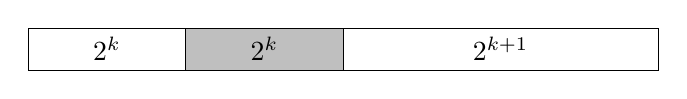
\begin{tikzpicture}[every node/.style={draw},
      small/.style={minimum width=2cm},
      large/.style={minimum width=4cm}]]
      \node[small] (m0) {$2^k$};
      \node[small,fill=gray!50] (m1) [right of=m0,xshift=1cm] {$2^k$};
      \node[large] (m2) [right of=m1,xshift=2cm] {$2^{k+1}$};
    \end{tikzpicture}
  \end{center}
  
  \reinitrand[counter=rand,first=3,last=5]
  A memória total disponível é $2^m$ unidades de memória. Se o valor de
  $k$ for igual a $\R$, responda às seguintes questões:
  
\begin{parts}
  \part Qual o valor de $m$?
  \part Qual a quantidade de memória que está ocupada em unidades de memória?
  \part Qual a quantidade de memória livre?
  \part Qual a quantidade total de memória?
\end{parts}
}

\def\PAGING{ 
  \question[3]~Dois processos possuem as seguintes
  páginas lógicas: $P1 = \{a, b, c\}, P2 = \{1, 2, 3, 4\}$. Supondo
  que o sistema operacional disp\~oe de 4 páginas físicas para alocar
  as páginas lógicas, fa\c{c}a um esboço gráfico para a ocupação das
  páginas lógicas que forem requisitadas na seguinte sequência:

  \reinitrand[counter=rand,first=1,last=4]
  \begin{center}
    $\{b,a,\R,\R,\R,\R,\R,\R,b,\R,a,\R,\R,\R,a,b,c\}$
  \end{center}
  utilizando os seguintes algoritmos de substituição de páginas:\\
 
  \begin{parts}
  %\part FIFO;
    \part Relógio;
    \part Segunda chance;
    \part LRU.
  \end{parts}\smallskip

  Calcule a taxa de falta de páginas (porcentagem de {\em page fault})
  para os algoritmos.

  \question[0,5] A tabela de páginas armazena informa\c{c}\~oes a
  respeito do mapeamento entre os endere\c{c}os l\'gicos e f\'isicos
  de mem\'oria. H\'a um campo de tamanho de 1 bit que informa se a
  p\'agina est\'a na mem\'oria f\'isica ou disco r\'igido e outro
  campo que marca se houve altera\c{c}\~ao no conte\'udo da p\'agina
  na mem\'oria f\'isica para que esta seja gravada em disco antes de
  ser retirada da tabela. Os bits que representam estes campos s\~ao
  chamados respectivamente de:

\begin{enumerate}[(a)]
{\item refer\^encia e sujeira.}
{\item validade e refer\^encia.}
{\item sujeira e validade.}
{\item validade e sujeira.}
{\item sujeira e refer\^encia.}
\end{enumerate}

\question[0,5] A tabela de p\'aginas localiza-se no (a):

\begin{enumerate}[(a)]
{\item Mem\'oria cache.}
{\item Registrador.}
{\item Disco Rígido.}
{\item Mem\'oria principal (DRAM).}
{\item Mem\'oria ROM.}
\end{enumerate}

}

\ifnum1=2
O que \'e a troca de mem\'oria ({\em swapping}) do espa\c{c}o de endere\c{c}amento de
processos?


\paragraph{Quest\~ao 6. (1,5 ponto)}
Defina as 4 entidades b\'asicas dos sistemas de
arquivos.

\paragraph{Quest\~ao \ex{}. (1,5 ponto)}
Defina e d\^e exemplos das classes gen\'ericas de dispositivos de entrada
e sa\'ida.

\fi

\lecture{Introdução ao Gerenciamento de Entrada e Saída (E/S)}{io:intro}

\title{\insertlecture}

\frame{\maketitle}

\part{\insertlecture}

\section{\insertlecture}

\begin{frame}{Entrada e Saída: E/S}  
  \usetikzlibrary{shapes}%add to preambule if the main file does not compile

\begin{tikzpicture}[control/.style={text width=1.65cm,align=center,font=\footnotesize,draw},
    every path/.style={draw},device/.style={fill=yellow,font=\scriptsize,minimum width=1cm},
    device connection/.style={dashed},
    disk/.style={black!80,font=\scriptsize,cylinder,minimum width=1.5cm,rotate=90,draw},
    os module/.style={minimum size=3.25cm,circle,red,line width=4,text width=2cm,draw},
    module label/.style={red,font=\bf\scriptsize}]

    \def\dx{3cm}
    \def\dy{2cm}
    
    \node[control] (proc) at (0,0) {processador};
    \node[control] (disk controller) at (\dx,0) {controladora de disco};
    \node[control] (usb controller) at (2*\dx,0) {controladora USB};
    \node[control] (video card) at (3*\dx,0) {placa de vídeo};
    \node[control,fill=green!40!black] (mem) at (1.5*\dx,-\dy) {memória};

    \path (proc) -- +(0,-0.5*\dy) -- +(3*\dx,-0.5*\dy) -- +(video card);
    \path (\dx,-0.5*\dy) -- +(disk controller);
    \path (2*\dx,-0.5*\dy) -- +(usb controller);
    \path (1.5*\dx,-0.5*\dy) -- +(mem);

    \node[disk] (hd) at (\dx,\dy) {disco rígido};
    \path[device connection] (disk controller) -- (hd);

    \node[device] (mouse) [above of=usb controller,yshift=\dy] {mouse};
    \node[device,fill=gray] (printer) [right of=mouse,xshift=.15*\dx] {impressora};
    \node[device,fill=yellow!70] (keyboard) [left of=mouse,xshift=-.15*\dx] {teclado};
    \path[device connection] (usb controller) -- (mouse);
    \path[device connection] (usb controller) -- (printer);
    \path[device connection] (usb controller) -- (keyboard);

    \node[device,fill=blue!30] (monitor) [above of=video card,yshift=.5*\dy] {\bf monitor};
    \path[device connection] (video card) -- (monitor);

    \node<2>[os module] (proc module) at (proc) {};
    \node<2>[module label] [above of=proc module,yshift=.5*\dy] {gerenciamento de processos};

    \node<3>[os module] (mem module) at (mem) {};
    \node<3>[module label] [below of=mem module,yshift=-.5*\dy] {gerenciamento de memória};

    \node<4>[module label,minimum width=7.5cm,dashed,draw] [above of=usb controller] {gerenciamento de entrada e saída (E/S)};
  \end{tikzpicture}

\end{frame}

\begin{frame}{Subsistema de entrada e saída}

  {\small Fonte:~\cite{ufrgs2008}}
  \begin{center}
    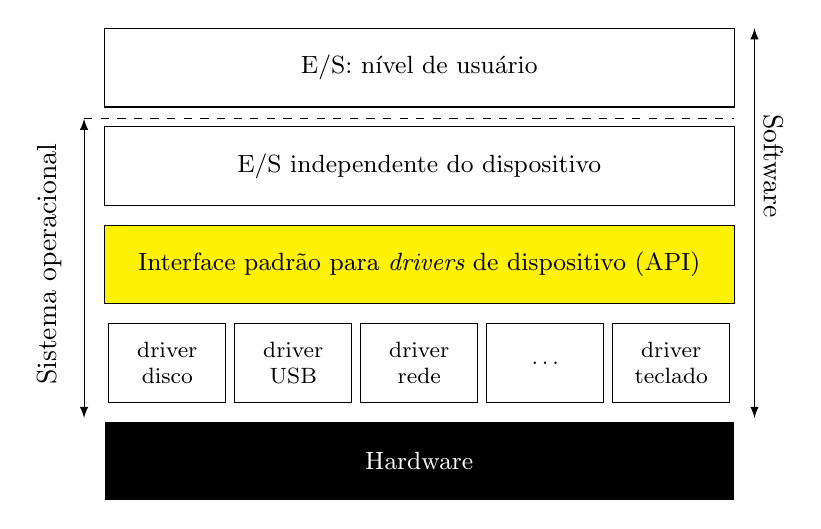
\begin{tikzpicture}[layer/.style={font=\small,minimum height=1cm,minimum width=8cm,draw},
      driver/.style={minimum height=1cm, align=center,font=\footnotesize,text width=1.25cm,draw},
      coda/.style={<->,>=latex}]
    
      \node[layer] (userlevel)  {E/S: nível de usuário};    
      \draw[dashed] (userlevel.west)+(-.25,-.65) -- +(8cm,-.65);
      \draw[coda] (userlevel.west)+(-.25,-.65) -- +(-.25,-4.45cm);
    
      \draw[coda] (userlevel.east)+(.25,.5) -- +(.25,-4.45cm);

      \node[layer] (io0) [below of=userlevel,yshift=-.25cm] {E/S independente do dispositivo};
      \node[layer,fill=yellow] (api) [below of=io0,yshift=-.25cm] {Interface padrão para {\em drivers} de dispositivo (API)};
    
      \foreach \x/\l in {-2/driver disco,-1/driver USB,0/driver rede,1/$\ldots$,2/driver teclado} {
        \node[driver] (driver\x) [below of=api, xshift=1.6*\x cm, yshift=-.25cm] {\l};
      }
      \node[white, fill=black, layer] (hardware) [below of=driver0, yshift=-.25cm] {Hardware};

      \node[rotate=90] [left of=driver-2,yshift=1.5cm,xshift=2.25cm] {Sistema operacional};
      \node [rotate=-90] [right of=io0,yshift=4.5cm,xshift=-1cm] {Software};

    \end{tikzpicture}
  \end{center}

\end{frame}

\begin{frame}{Dispositivos de entrada e saída}

  Além das abstrações de processos, espaços de endereçamento e arquivos,
  os SOs também controlam os dispositivos de E/S para:

  \begin{itemize}
  \item Emitir comandos para dispositivos;
  \item Interceptar interrupções e tratar erros;
  \item Atuar como interface entre os dispositivos e o restante do sistema.
  \end{itemize}

\end{frame}

\begin{frame}{Drivers de dispositivo}{Exemplo: driver de placa de rede}
  \begin{center}  
    
%%% Local Variables: 
%%% mode: latex
%%% TeX-master: "../notes"
%%% End: 


\def\w{2}
\def\h{1.5}
\def\xdelta{1.5}
\def\ydelta{1}
\begin{tikzpicture}
  \tikzset{every node/.style={text width=2cm,font={\footnotesize}},
  module/.style={rectangle,minimum height=1.5cm,draw}}
  \foreach \y/\l in {0/{Aplicação de rede},-2/{Subsistema de rede do
      SO},-4/{Driver da placa de rede},-6/{Placa de rede}} {
    \node[module] (\y) at (0,\y+\h) {\l};
  }
  \foreach \s/\d in {0/-2,-2/-4,-4/-6} {
    \path[<->,>=latex,draw] (\s) -- (\d);
  }

  \draw (-\xdelta,\ydelta) -- (\w+\xdelta,\ydelta) node[above]
  {\scriptsize Espaço
  do usuário};
\node [right of=-2,xshift=25mm] {Espaço do kernel};

  \draw (-\xdelta,-3.5) -- (\w+\xdelta,-3.5) node[text width=3cm,right] {Interface com o
    dispositivo de rede};
  \node [right of=-6,xshift=25mm] {Hardware};
\end{tikzpicture}
  \end{center}
\end{frame}

\begin{frame}{Classificação das camadas de E/S}
  
  \begin{block}<1->{Dispositivos de caracter}
    São dispositivos cujo fluxo de dados ocorre de forma sequencial,
    um byte após o outro.\\
    \smallskip
    Exemplo: teclado, porta serial.
  \end{block}

  \begin{block}<2->{Dispositivos de bloco}
    Os dados são acessados de forma aleatória em pedaços de 
    tamanho fixo chamado blocos.\\
    \smallskip
    Exemplo: Disco rígido, memória flash, disquete, leitor de Blu-ray.    
  \end{block}

  \begin{block}<3>{Dispositivos de rede} Os dados são recebidos e
    transmitidos em pacotes. \\\smallskip
    Exemplo: Interface de rede. 
  \end{block}
  
\end{frame}

\part{Interrupções e DMA}
\frame{\partpage}

\transition{Interrupções}{IRQ}

\begin{frame}{\insertlecture} 
  \begin{itemize}
  \item<1-> Interrupções permitem que o hardware sinalize o processador;
  \item<2-> Dispositivos de hardware geram interrupções assíncronas com respeito ao 
    relógio ({\it clock}) do processador;
  \item<3> Cada hardware possui um número de interrupção chamado IRQ
    ({\it interrupt request}). Alguns IRQs fixos para PC baseado em
    Intel são listados a seguir:
  \end{itemize}

  \begin{block}<3>{}
    \begin{center}
      \begin{tabular}[h]{c|l}\hline
        \color{red}IRQ &\hfil\color{red} dispositivo \\\hline
        0 & sinal de {\it clock} da placa-mãe \\
        1 & teclado \\
        7 & porta paralela \\
        11 & controlador USB\\\hline
      \end{tabular}
    \end{center}
  \end{block}
  
\end{frame}


\begin{frame}{\insertlecture}
  
  \begin{tikzpicture}[every node/.style={font=\tiny,text centered},
    ctr/.style={text width=1.75cm,draw}, 
    every path/.style={->,>=latex,draw},
    action/.style={text width=2cm,color={gray!70!black}}]

    \node<1-> (K) {\pgfuseimage{keyboard}};
    \node<2->[ctr] (CTRIRQ) [below of=K,yshift=-1cm] {controlador de interrupção};
    \node<3-> (P) [below of=CTRIRQ,yshift=-1cm] {\pgfuseimage{processor}};

    \node<4->[action] (A1) [right of=CTRIRQ, xshift=1.5cm] {processador interrompe o kernel};
    \node<5->[action] (A2) [right of=A1, xshift=1.5cm] {interrupção é manipulada};
    \node<6->[action] (A3) [right of=A2, xshift=1.5cm] {retorna para o código interrompido do kernel};

    \path<2-> (K) -- node[text width=1.2cm,left] {gera interrupção} (CTRIRQ);
    \path<3-> (CTRIRQ) -- (P);
    \path<4-> (P) -- (A1);
    \path<5-> (A1) -- (A2);
    \path<6-> (A2) -- (A3);
  \end{tikzpicture}

\end{frame}

\begin{frame}{Controle das interrupções}

  \begin{itemize}
  \item<1-> As interrupções podem ser desabilitadas para um processador 
    específico;
  \item<2-> Podem ser escolhidas números de IRQs para serem desabilitados 
    pelo SO;
  \item<3> Um mecanismo alternativo à interrupção é o acesso direto à
    memória.
  \end{itemize}
  
\end{frame}

% retirado de Linux Device Drivers
\transition{Acesso Direto à Memória}{DMA}

\begin{frame}{\insertlecture}

  \begin{itemize}
  \item<1-> O acesso direto à memória ou DMA ({\it Direct Memory Access})
    é o mecanismo de hardware que permite que periféricos transfiram
    sua E/S diretamente pela memória principal sem envolver o
    processador.
  \item<2-> O uso deste mecanismo a vazão de um dispositivo, pois boa parte 
    da sobrecarga computacional é eliminada.
  \end{itemize}

\end{frame}

\begin{frame}{Processo de transferência de dados, caso 1}{DMA}
  
  No caso 1, o processo pode ser resumido da seguinte forma:
  \begin{enumerate}
  \item<1-> Quando um processo chama uma função para transferência de
    dados, por exemplo {\tt read()} ou {\tt fread()}, o driver aloca
    um {\it buffer} de DMA e instrui o hardware a transferir seus
    dados para este {\it buffer}. O processo é colocado para dormir.
  \item<2-> O hardware escreve os dados no {\it buffer} e lança uma
    interrupção ao término.
  \item<3-> O manipulador de interrupção acessa os dados de entrada,
    responde à interrupção, acorda o processo, que em seguida pode ler
    os dados.
  \end{enumerate}

\end{frame}

%% from LDD pg 441
\begin{frame}{Processo de transferência de dados, caso 1}{DMA}

  O caso 2 ocorre quando o DMA é usado de forma assíncrona. Isto acontece 
  quando um hardware envia dados mesmo quando não há requisição. O processo 
  pode ser resumido da seguinte forma:
  \begin{enumerate}
  \item<1> O hardware lança uma interrupção para anunciar que chegaram
    novos dados.
  \item<2-> O manipulador de interrupção aloca um buffer e comunica ao 
    hardware onde transferir seus dados.
  \item<3-> O dispositivo periférico escreve os dados no {\it buffer}
    e lança outra interrupção ao término.
  \item<4-> O manipulador despacha os dados novos, acorda qualquer processo 
    associado, e se encarrega da liberação da memória utilizada.
  \end{enumerate}

\end{frame}

\transition{Dispositivos de bloco}{block}

\begin{frame}{\insertlecture}{Introdução}

  \begin{itemize}
  \item Os \alert{\insertlecture} fornecem acesso a dispositivos que
    transferem aleatoreamente blocos de tamanho fixo, tais como disco
    rígido, CD-ROM, DVD-ROM dentre outros.
  \item Os blocos frequentemente possuem o tamanho de \alert{4096
      bytes}, porém, este tamanho pode variar de acordo com a
    arquitetura e sistema de arquivos.
  \end{itemize}

  Drivers eficientes são críticos para performance.

\end{frame}


\begin{frame}{\insertlecture}
  {Conceitos essenciais}
  
  \begin{itemize}
  \item A menor unidade endereçável em um dispositivo de bloco é um \alert{setor}.
  \item O tamanho mais comum do setor é \alert{512} bytes. Porém, alguns dispositivos
    possuem tamanhos diferentes, por exemplo, muitos CD-ROMs possuem setores de 2-KB.
  \item Os blocos são armazenados temporariamente em um zona de memória chamada 
    \alert{\em buffer}, para ajuste entre as diferenças na velocidade de transferência entre
    as camadas dos subsistemas. \\
    \smallskip
    {\small Por exemplo, se a placa de rede suporta envio de blocos 
      de 4-KB, e o SO necessita enviar 64-KB, estes são armazenados no {\em buffer} até
      o término da transmissão.}

  \end{itemize}
        
\end{frame}

\part{Dispositivo de bloco}
\frame{\partpage}

\transition{Dispositivos de Bloco: Disco Rígido}{io:dev:block}

\begin{frame}{Busca em disco rígido}{\only<1>{Trilha}\only<2>{Setor}\only<3>{Cabeçote de leitura e escrita}}
  \begin{center}
    \input{../../chard-disk}
  \end{center}
\end{frame}

\transition{Escalonamento de disco}{diskScheduling}

\begin{frame}{Escalonamento das requisições de disco}
  
  \begin{itemize}
  \item O \alert{escalonador de disco} gerencia a fila de requisições
    dos dispositivos de bloco, decidindo qual requisição é despachada,
    com o objetivo de maximizar a performance global de E/S do
    sistema.
  \item O escalonadores de disco realizam 2 ações principais sobre as
    requisições para minimizar as buscas:
    \begin{itemize}
    \item \alert{Fusão}: agrupamento de 2 ou mais requisições ao mesmo bloco;
    \item \alert{Ordenação}: classifica as requisições de acordo com
      algum critério.
    \end{itemize}
  \end{itemize}
\end{frame}

\tikzset{plate/.style={}}

\begin{frame}{Algoritmos de escalonamento de disco}{FCFS}
  
  \alert{FCFS}({\em firt-come first-served}): as requisições são
  atendidas conforme a ordem de chegada na fila. Exemplo: 23, 89, 132,
  42, 187. No início o cabeçote está na posição 100.

  \bigskip
  \begin{tikzpicture}[move/.style={->,>=latex,thick,red!60!black, dotted,draw}]
    
    \draw[thick]  (-\textwidth/2,0) node[above] {0} -- (\textwidth/2,0) node[above] {199};
    \node (O) at (0,0) {};
    \node (h100) at (0,.2) {100};
    \node (r23) at (-.77*\textwidth/2,-1*.7) {23};
    \node (r89) at (-.11*\textwidth/2,-2*.7) {89};
    \node (r132) at (.32*\textwidth/2,-3*.7) {132};
    \node (r42) at (-.58*\textwidth/2,-4*.7) {42};
    \node (r187) at (.87*\textwidth/2,-5*.7) {187};

    \path[move] (O) -- (r23);
    \path[move] (r23) -- (r89);
    \path[move] (r89) -- (r132);
    \path[move] (r132) -- (r42);
    \path[move] (r42) -- (r187);

  \end{tikzpicture}

  \pause\footnotesize\hfil  total de trilhas = $77+66+43+90+145 = 421$ trilhas\bigskip

\end{frame}

\begin{frame}{Algoritmos de escalonamento de disco}{SSTS}
  \small
  \alert{SSTF} ({\em shortest seek time first}): as requisições
  são atendidas de acordo com o menor tempo de acesso, e são
  reordenadas constantemente, para levar em conta a posição atual do
  cabeçote, privilegiando os setores mais próximos à posição
  corrente na reordenação da fila de requisições.

  \begin{tikzpicture}[move/.style={->,>=latex,thick,red!60!black, dotted,draw}]
    
    \draw[thick]  (-\textwidth/2,0) node[above] {0} -- (\textwidth/2,0) node[above] {199};
    \node (O) at (0,0) {};
    \node (h100) at (0,.2) {100};
    \node (r89) at (-.11*\textwidth/2,-1*.7) {89};
    \node (r132) at (.32*\textwidth/2,-2*.7) {132};
    \node (r187) at (.87*\textwidth/2,-3*.7) {187};
    \node (r42) at (-.58*\textwidth/2,-4*.7) {42};
    \node (r23) at (-.77*\textwidth/2,-5*.7) {23};

    \path[move] (O) -- (r89);
    \path[move] (r89) -- (r132);
    \path[move] (r132) -- (r187);
    \path[move] (r187) -- (r42);
    \path[move] (r42) -- (r23);

  \end{tikzpicture}

  \bigskip

  \only<2>{\footnotesize\hfil total de trilhas =
    $11+43+55+145+19 = 273$ trilhas}

  \only<3>{\color{red}\small Desvantagem: Suscetível à postergação
    indefinida ({\em starvation}).}
\end{frame}
  
\begin{frame}{Algoritmos de escalonamento de disco}{SCAN}
  \footnotesize
  \alert{SCAN}: é uma variação do SSTF que se diferencia por
  adotar um sentido de varredura preferencial, como por exemplo do
  mais interno para o mais externo. Ao atingir o mais interno,
  inverte-se o sentido e novas requisições no sentido contrário são
  atendidas na próxima varredura. 
  
  \begin{tikzpicture}[move/.style={->,>=latex,thick,red!60!black, dotted,draw}]
    
    \draw[thick]  (-\textwidth/2,0) node[above] {0} -- (\textwidth/2,0) node[above] {199};
    \node (O) at (0,0) {};
    \node (h100) at (0,.2) {100};
    \node (r89) at (-.11*\textwidth/2,-1*.6) {89};
    \node (r42) at (-.58*\textwidth/2,-2*.6) {42};
    \node (r23) at (-.77*\textwidth/2,-3*.6) {23};
    \node (left) at (-\textwidth/2,-4*.6) {0};
    \node (r132) at (.32*\textwidth/2,-5*.6) {132};
    \node (r187) at (.87*\textwidth/2,-6*.6) {187};

    \path[move] (O) -- (r89);
    \path[move] (r89) -- (r42);
    \path[move] (r42) -- (r23);
    \path[move] (r23) -- (left);
    \path[move] (left) -- (r132);
    \path[move] (r132) -- (r187);
  \end{tikzpicture}
  
  \bigskip

  \only<2>{\footnotesize\hfil total de trilhas =
    $11+47+19+23+132+55 = 287$ trilhas}

  \only<3>{Também é conhecido como algoritmo do \alert{elevador}.}

\end{frame}

\begin{frame}{Algoritmos de escalonamento de disco}{C-SCAN}

  \alert{C-SCAN}: variação do SCAN que se diferencia por adotar
  o sistema de varredura em somente uma direção. Por exemplo, se o
  cabeçote atingir o cilindro mais interno, é então reposicionado
  no cilindro mais externo e a varredura é realizada novamente.

  \begin{tikzpicture}[move/.style={->,>=latex,thick,red!60!black, dotted,draw}]
    
    \draw[thick]  (-\textwidth/2,0) node[above] {0} -- (\textwidth/2,0) node[above] {199};
    \node (O) at (0,0) {};
    \node (h100) at (0,.2) {100};
    \node (r89) at (-.11*\textwidth/2,-1*.5) {89};
    \node (r42) at (-.58*\textwidth/2,-2*.5) {42};
    \node (r23) at (-.77*\textwidth/2,-3*.5) {23};
    \node (left) at (-\textwidth/2,-4*.5) {0};
    \node (right) at (\textwidth/2,-5*.5) {199};
    \node (r187) at (.807*\textwidth/2,-6*.5) {187};
    \node (r132) at (.32*\textwidth/2,-7*.5) {132};

    \path[move] (O) -- (r89);
    \path[move] (r89) -- (r42);
    \path[move] (r42) -- (r23);
    \path[move] (r23) -- (left);
    \path[move] (left) -- (right);
    \path[move] (right) -- (r187);
    \path[move] (r187) -- (r132);
  \end{tikzpicture}

  \bigskip

  \only<2>{\footnotesize\hfil total de trilhas =
    $11+47+19+23+199+12+55 = 366$ trilhas}

\end{frame}


\begin{frame}
  
  \begin{thebibliography}{5}
  \bibitem[Oliveira, 2008]{ufrgs2008}
    {\em Sistemas Operacionais}.
    \newblock Rômulo Silva de Oliveira, Alexandre da Silva Carissimi e 
    Simão Sirineo Roscani.
    \newblock Editora Bookman, 2008.
  
  \bibitem[LKD3]{lkd3} 
    {\em Linux Kernel Development}.
    \newblock Robert Love.
    \newblock Addison Wesley, 3rd edition, 2010.

  \bibitem[LDD3]{ldd3} 
    {\em Linux Device Drivers}.
    \newblock Jonathan Corbet, Alessandro Rubini, Greg Kroah-Hartman.
    \newblock O'Reilly, 3rd edition, 2010.

  \bibitem[WAGmob]{wagmob} 
    {\em Operating System 101}.
    \newblock WAGmob.

  \bibitem[Garrido, 2008]{garrido2008}
    {\em Principles of Modern Operating Systems}.
    \newblock José M.\ Garrido, Richard Schlesinger.
    \newblock Jones and Bartlett Publishers, 2008.

  \end{thebibliography}

\end{frame}


\lecture{Exercício de Escalonamento de E/S}{io:exercise}

\begin{frame}{Exercício}

  \begin{enumerate}
  \item Dada as seguintes sequências de requisições para um 
    disco com $100$ trilhas:
    \begin{center}
      $44, 20, 95, 4, 50, 52, 47, 61, 87, 25$,
    \end{center}
    onde a posição atual dos cabeçotes é $50$, calcule a deslocamento
    de dos cabeçotes para atender às requisições utilizando os
    seguintes algoritmos de escalonamento de E/S:
    \begin{enumerate}
    \item FCFS;
    \item SSTF;
    \item SCAN;
    \item C-SCAN.
    \end{enumerate}
  \end{enumerate}
  
\end{frame}

\end{document}

\transition{RAID}{RAID}

\begin{frame}{RAID 0}
  
  \includegraphics[scale=.3]{raid0.png}

\end{frame}


\begin{frame}{RAID 1}
  
  \includegraphics[scale=.3]{raid1.png}

\end{frame}


\begin{frame}{RAID 5}
  
  \includegraphics[scale=.3]{raid5.png}

\end{frame}

\begin{frame}{RAID 0+1}
  
  \includegraphics[scale=.3]{raid01.png}

\end{frame}



 
\section*{Sistema de Arquivos}

\paragraph{estatística de E/S} Use o comando {\tt stat} para extrair as seguintes
informações dos arquivos:\\

\begin{minipage}{.5\textwidth}
  \begin{itemize}
  \item Tamanho do arquivo;
  \item Número de blocos;
  \item Tamanho de cada bloco;
  \item Tipo de arquivo;
  \end{itemize}
\end{minipage}
\begin{minipage}{.5\textwidth}
  \begin{itemize}
  \item Número do inode;
  \item Permissões;
  \item Acesso.
  \end{itemize}
\end{minipage}


\end{document}
"
% generates the article version of the document
\ifdefined\isarticle
  \documentclass[a4paper]{article}
  \usepackage{beamerarticle}
  \usepackage{fullpage}
\else
  % ignorenonframetext as argument to beamer causes no page of output
  \documentclass[]{beamer}
  \usecolortheme{beaver}
  \setbeamercovered{highly dynamic}
\fi

\usepackage{fontspec} % use XeLaTeX
\usepackage[]{polyglossia}
\setdefaultlanguage{brazil}
\usepackage{hyperref}
\hypersetup{colorlinks=true,linkcolor=blue,anchorcolor=blue,urlcolor=blue}
\usepackage{pgf,tikz} % Draw figures
\usetikzlibrary{arrows,automata,calc,chains,circuits,graphs,positioning,shapes.gates.logic.US,shapes,trees}
\usepackage{circuitikz}
  \usepackage{listings}
  \lstset{language=C,inputencoding=utf8,basicstyle=\footnotesize, 
    flexiblecolumns=true, numbers=left, numberstyle=\tiny\color{gray}, 
    commentstyle=\scriptsize\color{black!50},mathescape}
  
  \usepackage{ifthen} % \ifthenelse

  % Definitions
  \author{Adriano J. Holanda}%\\{\scriptsize \url{http://holanda.xyz}}}
  \def\array{vetor}
  \def\bigO#1{\mathcal{O}(#1)}
  \def\bug#1{{\it bug#1\/}}
  % C letter
  \font\ninerm=cmr9
  \let\mc=\ninerm
  \def\CEE{{\mc C\spacefactor1000}}

  \def\boxset{
    \tikzset{box/.style={rectangle,minimum width=.5cm,draw},
      index/.style={minimum width=.5cm}}
  }

%%%%%%%%%%%%%%%%%%%%%%%%%%%%%%%%%%%%%%%%%%%%%%%%%%%%%%%%%%%%%%%%%%%%%%%%%%%%%%% 
\pgfdeclareimage[width=2.5cm]{keyboard}{teclado.png}
\pgfdeclareimage[width=1.5cm]{processor}{processor.png}

\begin{document}

%\input proc
%\input thread
%\input sched
\input lock
%\input deadlock
%\input mem
%\input address-space
%\input vmem
%\input io
%\input raid
%\input fs
%\input vfs
%\input ext4
%\input fs-win
\end{document}
